\documentclass[11pt,a4paper]{article}
\usepackage[T1]{fontenc}
\usepackage[utf8]{inputenc}
\usepackage{lmodern}
\usepackage{microtype}
\usepackage[margin=28mm,headheight=14pt]{geometry}
\usepackage{amsmath,amssymb,amsthm,mathtools,bm}
\usepackage{booktabs,array,tabularx,longtable}
\usepackage{graphicx}
\usepackage{xcolor}
\usepackage{enumitem}
\usepackage{fancyhdr}
\usepackage{hyperref}
\usepackage[backend=biber,style=alphabetic,sorting=nyt,maxbibnames=6]{biblatex}
\addbibresource{references.bib}
\hypersetup{colorlinks=true,linkcolor=blue!45!black,citecolor=blue!45!black,urlcolor=blue!50!black,pdftitle={Joint Local Sieves and First-Arrival Dynamics of Goldbach Imbalances},pdfauthor={Paul A. Bilokon}}
\setlength{\parskip}{4pt}
\setlength{\parindent}{0pt}
\setlist[itemize]{leftmargin=1.5em,itemsep=2pt,topsep=2pt}
\renewcommand{\arraystretch}{1.13}
\pagestyle{fancy}
\fancyhf{}
\fancyhead[L]{\footnotesize Joint sieves and Goldbach first arrivals}
\fancyhead[R]{\footnotesize Working manuscript, October 2026}
\fancyfoot[C]{\thepage}
\newtheorem{theorem}{Theorem}[section]
\newtheorem{proposition}[theorem]{Proposition}
\newtheorem{corollary}[theorem]{Corollary}
\newtheorem{lemma}[theorem]{Lemma}
\theoremstyle{definition}
\newtheorem{definition}[theorem]{Definition}
\newtheorem{remark}[theorem]{Remark}
\newcommand{\PP}{\mathbb P}
\newcommand{\ind}{\mathbf 1}
\newcommand{\E}{\mathbb E}
\newcommand{\Prob}{\mathbb P\mathrm r}
\newcommand{\F}{\mathcal F}
\newcommand{\ZZ}{\mathbb Z}
\newcommand{\nuell}{\nu_{\ell}}
\newcommand{\Nset}{\mathcal N_X}
\title{\textbf{Joint Local Sieves and First-Arrival Dynamics\\of Goldbach Imbalances}\\[5pt]\large Exact Modular Correlations, Void Probabilities,\\Factorial Cumulants and a Conditional Poisson Law}
\author{Paul A. Bilokon\\\small Mathematical working paper}
\date{18 October 2026}
\begin{document}
\maketitle
\begin{abstract}
We investigate the distance from the centre of an even integer to its nearest Goldbach representation, emphasizing the guaranteed-reset progression $N\equiv10\pmod{60}$.  Candidate representations occur at the lattice sites $N/2\pm6j$, and the first successful site defines a first-arrival process in the normalized imbalance interval.  For arbitrary finite families of candidate sites we prove an exact Chinese-remainder-theorem density formula for surviving local congruence classes.  The associated two-site multiplier is explicitly repulsive in the generic case and attractive when $i\equiv\pm j\pmod\ell$.  A four-site selection gives an exact joint non-occurrence theorem modulo $7$.  Computations over $483{,}333$ even targets in $[10^6,3\cdot10^7]$ compare sieve-predicted pair correlations with actual prime pairs and examine the void probability using the first three factorial cumulants.  We formulate and prove a conditional moment-to-Poisson theorem that isolates the stronger, presently unavailable, high-order prime-tuple estimates required for an exponential first-arrival law.  All finite residue-count identities are unconditional; numerical fits, heuristic Euler products, and asymptotic conjectures are labeled separately.
\end{abstract}
\vspace{-5pt}
\noindent\textbf{Keywords:} Goldbach problem; imbalance metric; prime tuples; singular series; sieve correlations; factorial cumulants; Poisson approximation.\\
\textbf{MSC 2020:} 11P32, 11N36, 11N05, 60G55.

\section{Goldbach intersections and the first-arrival lattice}
Let $S(n)=\{p\in\PP:2n-p\in\PP\}$, so that every $p\in S(n)$ contributes an ordered Goldbach representation of $2n$.  The Goldbach intersection $I_k(n)=S(n)\cap S(n-k)$ describes a common prime endpoint and a complementary prime pair of difference $2k$.  Its imbalance-space dynamics was considered in the companion working manuscript \cite{Bilokon2026Dynamics}; here we investigate the first occupied central site and its arithmetic correlations.

For an even integer $N=2m$, put
\begin{equation}\label{eq:distance}
 d(N)=\min_{\substack{p,q\in\PP\\p+q=N}}\frac{|q-p|}{2},\qquad
 \delta_{\min}(N)=\frac{d(N)}m=\frac{2d(N)}N.
\end{equation}
If no representation exists, we set $d(N)=+\infty$.  The quantity $d(N)$ is the first occupied distance from the midpoint, whereas $\delta_{\min}$ is the corresponding first-arrival imbalance on $[0,1]$.

We focus on the progression
\begin{equation}\label{eq:progression}
 N=60s+10,\quad s\ge1,\qquad m=\frac N2=30s+5.
\end{equation}
It provides guaranteed complete resets of common-prime endpoints because $N-5=5(12s+1)>5$ is composite.  More precisely, the earlier elementary congruence argument gives $S((N-2)/2)\cap S(N/2)=\varnothing$: no prime endpoint is transported unchanged from midpoint $m-1$ to midpoint $m$.  This does \emph{not} assert that either row is empty.

Every nonexceptional Goldbach representation of $N$ has its prime summands congruent to $5\pmod6$; hence it is
\begin{equation}\label{eq:candidates}
 p_j=m-6j,\quad q_j=m+6j,\qquad j=1,2,\ldots,\quad p_j\ge5.
\end{equation}
The special representation $3+(N-3)$, if present, lies at distance $m-3$ and can be checked separately.  Define
\begin{equation}\label{eq:Aj}
 A_j(N)=\ind_{\PP}(m-6j)\ind_{\PP}(m+6j),\qquad
 J_*(N)=\min\{j\ge1:A_j(N)=1\}.
\end{equation}
For targets whose nearest representation is nonexceptional, $d(N)=6J_*(N)$.  Since $5\mid m$, every site $j\equiv0\pmod5$ is impossible (when $m-6j\ge5$ is larger than $5$): the two endpoints are multiples of $5$.  We thus work with $j\ge1$, $5\nmid j$.

\section{First-arrival scaling and the factorization of the target}
The sieve data from the preceding first-arrival investigation contain all $499{,}999$ targets $N=60s+10$ between $70$ and $29{,}999{,}950$.  Every tested target has a Goldbach representation.  These facts are \emph{finite computational observations}. They are not asserted for arbitrary $N$.  The nearest half-gap $d(N)$ can be determined exactly by testing the pairs \eqref{eq:candidates} in increasing order of $j$, checking the exceptional pair involving $3$ only if needed.

\begin{table}[ht]
\centering\small
\begin{tabular}{@{}rrrrr@{}}
\toprule
Range of $N$ & Targets & Median $d(N)$ & Mean $d(N)$ & Mean $d/\log^2(N/2)$\\
\midrule
$10^4\le N<10^5$ & 1,500 & 36 & 46.32 & 0.453\\
$10^5\le N<10^6$ & 15,000 & 54 & 74.53 & 0.485\\
$10^6\le N<10^7$ & 150,000 & 78 & 107.14 & 0.496\\
$10^7\le N\le3\cdot10^7$ & 333,333 & 96 & 129.12 & 0.500\\
\bottomrule
\end{tabular}
\caption{Nearest-pair distances from exhaustive prime-sieve enumeration on the indicated arithmetic progression. The last column uses the natural logarithm.}
\label{tab:scaling}
\end{table}

\begin{figure}[ht]
\centering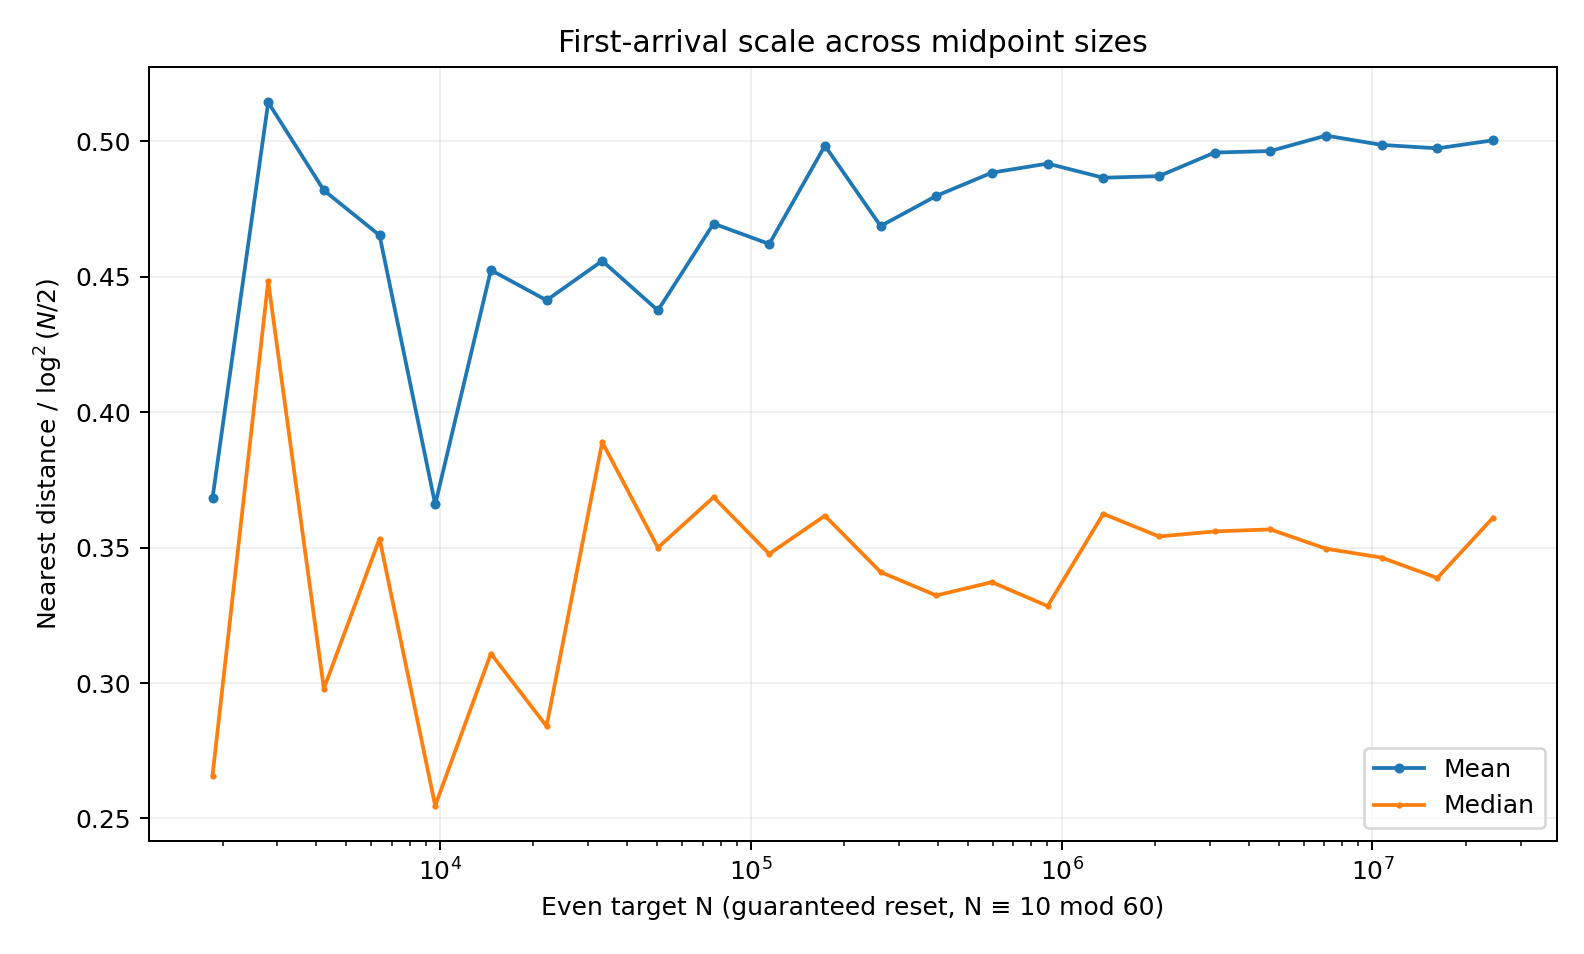
\includegraphics[width=.89\linewidth]{figures/first_arrival_scaling.png}
\caption{First-arrival scaling across increasing target ranges. The absolute half-gap grows slowly, while the normalized imbalance $\delta_{\min}=2d/N$ diminishes.}
\label{fig:scaling}
\end{figure}

The classical singular-series adjustment $H(N)$ defined in \eqref{eq:H} below suggests that a divisor $\ell\mid N$ enhances local admissibility by $(\ell-1)/(\ell-2)$. In the subset $N\ge10^6$, we measure:
\begin{table}[ht]
\centering\small
\begin{tabular}{@{}rrrr@{}}
\toprule
Prime $\ell$ & $\E[d/\log^2(N/2)\mid\ell\nmid N]$ & $\E[d/\log^2(N/2)\mid\ell\mid N]$ & Observed ratio\\
\midrule
7 & 0.5117 & 0.4190 & 0.819\\
11 & 0.5041 & 0.4427 & 0.878\\
13 & 0.5025 & 0.4506 & 0.897\\
\bottomrule
\end{tabular}
\caption{Empirical conditional means. The corresponding naive inverse-singular-series ratios are $(\ell-2)/(\ell-1)$: $0.833$, $0.900$, $0.917$.}
\label{tab:divisors}
\end{table}

These figures motivate the scale $d(N)/\log^2(N/2)$ and the further singular-series normalization $Z(N)$ in \eqref{eq:Z}. The sample mean of $Z$ for $N\ge10^6$ is $0.928$, with median $0.660$, while the standard exponential law has mean $1$ and median $\log2\approx0.693$. The large-distance tail is somewhat lighter than a simple exponential fit in the observed range. For example, the observed survival frequencies $\Pr(Z>1)$ and $\Pr(Z>2)$ are $0.3420$ and $0.1121$, versus $e^{-1}=0.3679$ and $e^{-2}=0.1353$.  The term ``probability'' here refers to choosing $N$ uniformly from the finite sample, not to a theorem about an asymptotic distribution.

\begin{figure}[ht]
\centering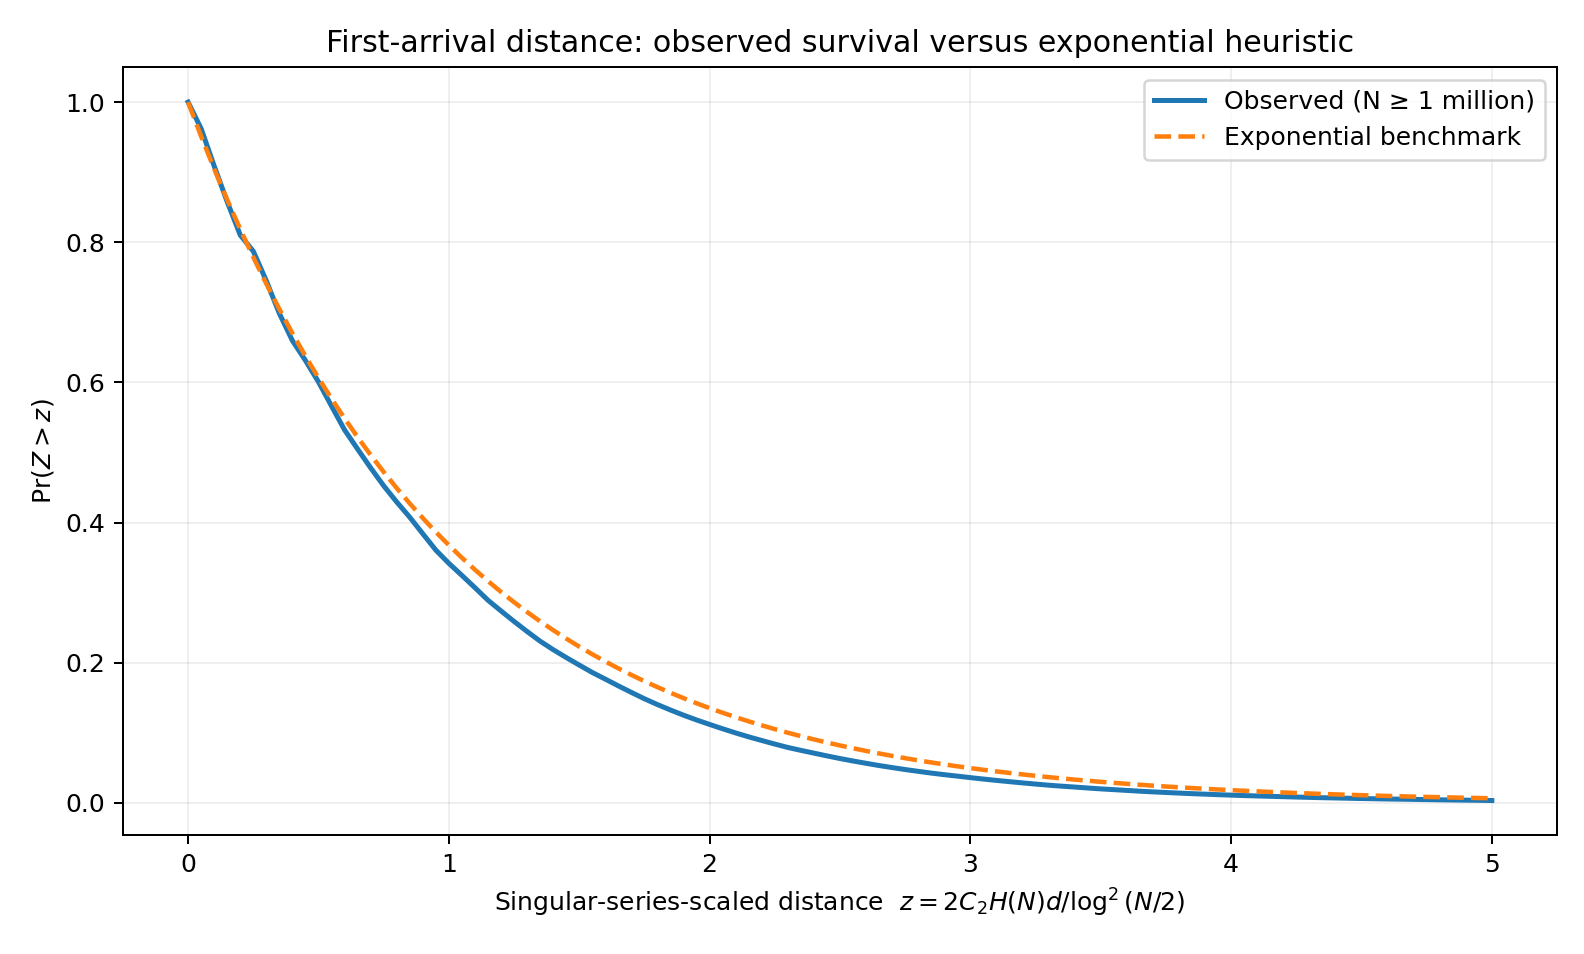
\includegraphics[width=.86\linewidth]{figures/first_arrival_survival.png}
\caption{Finite empirical survival for the singular-series-scaled first-arrival variable, against the exponential heuristic. This comparison motivates the joint-sieve and cumulant analysis below.}
\label{fig:firstsurvival}
\end{figure}

The most extreme half-gap in this computed progression occurs at $N=12{,}237{,}430$ and equals $d(N)=1{,}512$, from the pair $6{,}117{,}203+6{,}120{,}227$. Its normalized imbalance is nevertheless only about $2.47\cdot10^{-4}$. The arithmetic and normalized geometric scales must therefore be kept separate.

\section{Exact local arithmetic: one and several candidates}
Choose a prime $\ell\ge7$ and keep an index $j$ fixed.  For a candidate pair to have neither endpoint divisible by $\ell$, it is necessary that
\begin{equation}\label{eq:forbidden}
 m\not\equiv \pm6j\pmod\ell.
\end{equation}
As $s$ varies in \eqref{eq:progression}, the midpoint $m=30s+5$ runs through every residue modulo $\ell$.  Consequently all probabilities in this section are \emph{exact uniform residue frequencies}, not assertions that primes behave randomly.

\begin{definition}
For a finite, nonempty set $\mathcal J\subset\ZZ_{\ge1}$ of eligible indices ($5\nmid j$ for $j\in\mathcal J$), define
\[
 \F_\ell(\mathcal J)=\bigcup_{j\in\mathcal J}\{6j,-6j\}\pmod\ell,
 \qquad \nu_\ell(\mathcal J)=|\F_\ell(\mathcal J)|.
\]
For a singleton or pair we abbreviate $\nu_\ell(j)$ and $\nu_\ell(i,j)$.
\end{definition}

\begin{proposition}[Finite CRT sieve]\label{prop:CRT}
Let $M$ be squarefree with all prime divisors at least $7$.  Among $s\bmod M$, the exact fraction for which no candidate endpoint at any index $j\in\mathcal J$ is divisible by any prime factor of $M$ equals
\begin{equation}\label{eq:CRT}
 \prod_{\ell\mid M}\left(1-\frac{\nu_\ell(\mathcal J)}\ell\right).
\end{equation}
In particular, if $\nu_\ell(\mathcal J)=\ell$ for some $\ell\mid M$, the fraction vanishes.
\end{proposition}
\begin{proof}
Modulo a fixed $\ell$, precisely $\nu_\ell(\mathcal J)$ values of $m$ are excluded by \eqref{eq:forbidden}, leaving $\ell-\nu_\ell(\mathcal J)$ possibilities. Since $m=30s+5$ is a bijective affine map modulo $\ell$, the same count applies to $s$. The Chinese remainder theorem multiplies the admissible counts over the factors of $M$. Dividing by $M$ proves the claim.
\end{proof}

\begin{proposition}[Exact local two-site multiplier]\label{prop:ratio}
For distinct eligible indices $i,j$, the local ratio between joint survival and the product of individual survival frequencies is
\begin{equation}\label{eq:ratio}
 R_\ell(i,j)=\frac{1-\nu_\ell(i,j)/\ell}
 {(1-\nu_\ell(i)/\ell)(1-\nu_\ell(j)/\ell)}.
\end{equation}
If $\ell\nmid ij$ and $i\not\equiv\pm j\pmod\ell$, then
\begin{equation}\label{eq:repulsion}
 R_\ell(i,j)=\frac{\ell(\ell-4)}{(\ell-2)^2}
 =1-\frac4{(\ell-2)^2}<1.
\end{equation}
If $\ell\nmid ij$ and $i\equiv\pm j\pmod\ell$, then
\begin{equation}\label{eq:attraction}
 R_\ell(i,j)=\frac\ell{\ell-2}>1.
\end{equation}
\end{proposition}
\begin{proof}
If neither index is zero and they are distinct up to sign, the four residues $\pm6i,\pm6j$ are distinct, so $\nu_\ell(i,j)=4$ while both marginals have $\nu_\ell=2$.  If the indices agree up to sign, the joint forbidden set has two elements.  Substitution gives the formulas.  If an index vanishes modulo $\ell$, the general formula \eqref{eq:ratio} still applies, with singleton $\nu_\ell=1$.
\end{proof}

The crucial resonance condition is $\ell\mid(i-j)(i+j)$, outside the exceptional cases $\ell\mid ij$.  Thus the local environment generally discourages simultaneous survival, while certain arithmetically determined separations favor it.

\begin{theorem}[A joint obstruction to four candidates]\label{thm:four}
For every sufficiently large $N\equiv10\pmod{60}$,
\begin{equation}\label{eq:forbiddenfour}
 A_1(N)A_2(N)A_3(N)A_7(N)=0.
\end{equation}
\end{theorem}
\begin{proof}
Modulo $7$, the set $\{\pm1,\pm2,\pm3,\pm7\}$ is all of $\ZZ/7\ZZ$. Since $6$ is invertible modulo $7$, the corresponding excluded midpoint residues also cover every residue. At least one candidate has an endpoint divisible by $7$; when $N$ is sufficiently large that all examined endpoints exceed $7$, that endpoint is composite.
\end{proof}

\begin{remark}
The residue obstruction \eqref{eq:forbiddenfour} is an exact exclusion of simultaneous \emph{successes}.  It says nothing by itself about how likely a long run of \emph{failures} is.  In particular, finite-modulus survival does not certify actual primality, and local admissibility alone cannot prove a Goldbach representation.
\end{remark}

\section{Truncated singular-series predictors}
The traditional Hardy--Littlewood singular series for even $N$ contains the enhancement factor
\begin{equation}\label{eq:H}
 H(N)=\prod_{\substack{\ell\mid N\\\ell>2}}\frac{\ell-1}{\ell-2},
 \qquad C_2=\prod_{\ell>2}\left(1-\frac1{(\ell-1)^2}\right)
 \approx0.6601618158,
\end{equation}
where $C_2$ is the twin-prime constant \cite{HardyLittlewood1923,GoldstonHuntsNgotiaoco2017}.  These factors motivate, but do not prove, the prime-pair first-arrival model.

For a cutoff $L\ge7$, let
\begin{align}
 W_L(j)&=\prod_{\substack{7\le\ell\le L\\\ell\in\PP}}
 \frac{1-\nu_\ell(j)/\ell}{(1-1/\ell)^2}, \label{eq:weight}\\
 R_L(i,j)&=\prod_{\substack{7\le\ell\le L\\\ell\in\PP}}R_\ell(i,j).\label{eq:prodR}
\end{align}
The $W_L$ are relative marginal sieving weights, while $R_L$ predicts joint/marginal correlation. For fixed distinct indices, the infinite product converges: its generic factors differ from one by $O(\ell^{-2})$, and nongeneric factors occur only at primes dividing finitely many fixed integers. This convergence concerns the \emph{arithmetic factors}, not a proven asymptotic for prime-pair correlations.

For separation $h$ and finite cutoff $J$, the particular weighted predictor used here is
\begin{equation}\label{eq:weighted}
 \mathcal R_{L,J}(h)=
 \frac{\displaystyle\sum_{\substack{1\le j<j+h\le J\\5\nmid j(j+h)}}
 W_L(j)W_L(j+h)R_L(j,j+h)}
 {\displaystyle\sum_{\substack{1\le j<j+h\le J\\5\nmid j(j+h)}}
 W_L(j)W_L(j+h)}.
\end{equation}
It has no fitted free parameter. We take $J=120$, $L=10{,}000$ for the comparison below.

\section{A reproducible prime experiment}
Define the finite target sample
\begin{equation}\label{eq:sample}
 \mathcal N=\{N:10^6\le N\le3\cdot10^7,\ N\equiv10\pmod{60}\}.
\end{equation}
There are exactly $|\mathcal N|=483{,}333$ targets.  The accompanying C++ programs sieve primes up to $30$ million and evaluate $A_j(N)$ for $1\le j\le120$.  For each eligible index $j$, let $\widehat p_j=|\mathcal N|^{-1}\sum_{N\in\mathcal N}A_j(N)$ and let $\mathcal P_h=\{j:1\le j<j+h\le120,\ 5\nmid j(j+h)\}$.  We report
\begin{equation}\label{eq:empirical}
 \widehat R(h)=
 \frac{\displaystyle\frac{1}{|\mathcal P_h||\mathcal N|}\sum_{j\in\mathcal P_h}\sum_{N\in\mathcal N}A_j(N)A_{j+h}(N)}
 {\displaystyle\frac1{|\mathcal P_h|}\sum_{j\in\mathcal P_h}\widehat p_j\widehat p_{j+h}}.
\end{equation}
Here the denominator uses \emph{position-specific} marginal hit rates. This avoids confusing changes in marginal success probabilities with pair dependence.

\begin{table}[ht]
\centering\small
\begin{tabular}{@{}rrr@{}}
\toprule
$h$ & Empirical $\widehat R(h)$ & Local $\mathcal R_{10000,120}(h)$\\
\midrule
1 & 0.8780 & 0.8742\\
2 & 0.8760 & 0.8666\\
3 & 0.8997 & 0.8837\\
5 & 0.8976 & 0.8898\\
7 & \textbf{1.2801} & \textbf{1.2667}\\
10 & 0.8847 & 0.8780\\
11 & \textbf{1.0887} & \textbf{1.0818}\\
12 & 0.8781 & 0.8750\\
14 & 1.2567 & 1.2500\\
\bottomrule
\end{tabular}
\caption{Joint/marginal relative frequencies on the sample \eqref{eq:sample}. The right column is a truncated Euler-product \emph{prediction}, not a theorem about prime tuples.}
\label{tab:corr}
\end{table}

\begin{figure}[ht]
\centering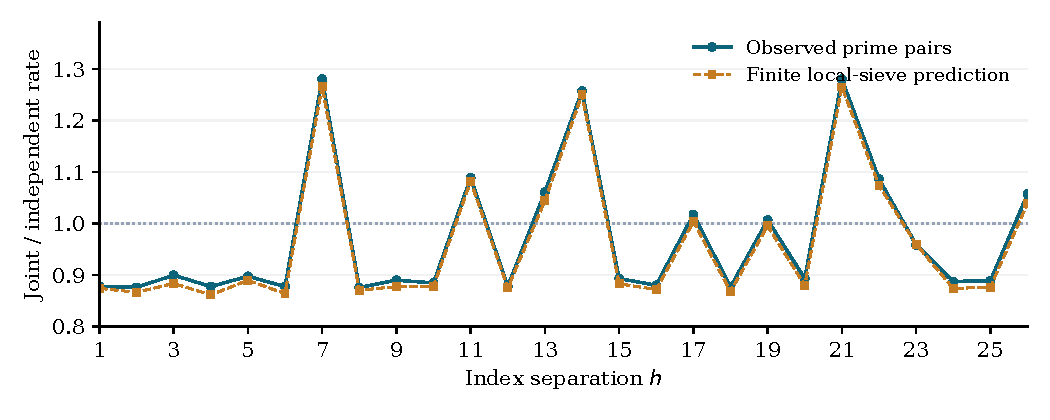
\includegraphics[width=.92\linewidth]{figures/correlation.pdf}
\caption{The empirical correlation ratio and the modular prediction for $h=1,\ldots,26$. Resonances at $h=7,14,21$ and $h=11,22$ are visible.}
\label{fig:corr}
\end{figure}
The numerical agreement includes the sign and approximate magnitude of several resonances.  It is evidence for a prime-tuple heuristic in this finite range, not an error estimate valid for all $N$.

\section{Void events, factorial cumulants and first arrival}
Let
\begin{equation}\label{eq:VJ}
 V_J(N)=\sum_{j=1}^J A_j(N),\qquad
 \widehat P_J(0)=\frac1{|\mathcal N|}\#\{N\in\mathcal N:V_J(N)=0\}.
\end{equation}
An empty window means that no nonexceptional central Goldbach pair was found among its first $J$ candidate sites. If $J_*(N)$ exists, then $\{J_*(N)>J\}=\{V_J(N)=0\}$.

For any nonnegative integer-valued random variable $V$, let $(V)_r=V(V-1)\cdots(V-r+1)$ and $\kappa_r$ denote its factorial cumulants.  The first three are
\begin{align}
 \kappa_1&=\mu=\E V,\nonumber\\
 \kappa_2&=\E(V)_2-\mu^2=\operatorname{Var}(V)-\mu,\label{eq:cums}\\
 \kappa_3&=\E(V)_3-3\E(V)_2\mu+2\mu^3.\nonumber
\end{align}
For finite $J$ the void probability obeys the exact inclusion--exclusion identity
\begin{equation}\label{eq:IE}
 \Prob(V_J=0)=\sum_{r=0}^J\frac{(-1)^r}{r!}\E (V_J)_r.
\end{equation}
Formally, the factorial cumulant expansion of $\log\E z^{V_J}$ at $z=1$ suggests the successive \emph{approximations}
\begin{align}
 P_J^{\mathrm{Pois}}&=e^{-\mu_J},\nonumber\\
 P_J^{(2)}&=\exp(-\mu_J+\kappa_2/2),\label{eq:approx}\\
 P_J^{(3)}&=\exp(-\mu_J+\kappa_2/2-\kappa_3/6).\nonumber
\end{align}
Truncating at $z=0$ is not automatically justified by a convergent infinite expansion; we use \eqref{eq:approx} as finite-sample models, not as rigorous upper or lower bounds.

\begin{table}[ht]
\centering\small
\begin{tabular}{@{}rrrrr@{}}
\toprule
$J$ & Actual $\widehat P_J(0)$ & Poisson & Second order & Third order\\
\midrule
5 & 0.795992 & 0.804223 & 0.796564 & 0.796039\\
10 & 0.623951 & 0.639902 & 0.625280 & 0.624082\\
20 & 0.378267 & 0.402409 & 0.380856 & 0.378703\\
40 & 0.137466 & 0.158687 & 0.140493 & 0.138413\\
60 & 0.050317 & 0.062539 & 0.051917 & 0.050759\\
100 & 0.006687 & 0.009735 & 0.007278 & 0.006889\\
\bottomrule
\end{tabular}
\caption{Observed frequency of no successful central pair, and factorial-cumulant approximations \eqref{eq:approx}. All values are finite-sample estimates on $\mathcal N$.}
\label{tab:void}
\end{table}

\begin{figure}[ht]
\centering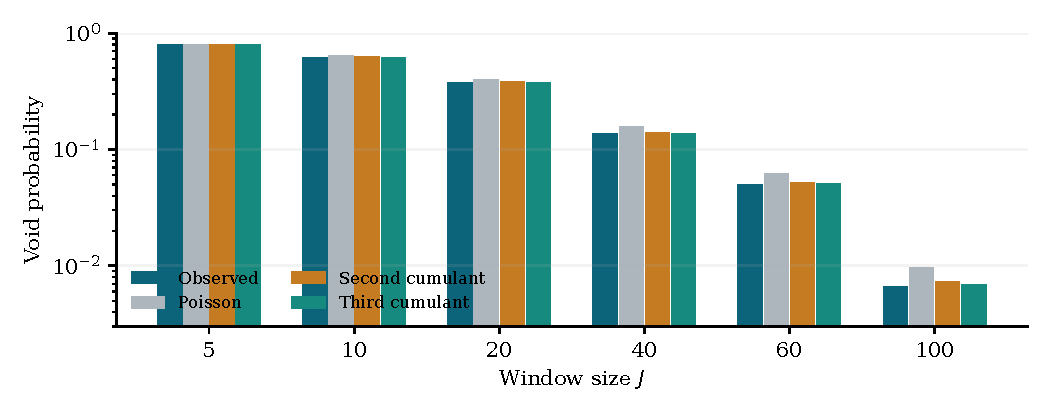
\includegraphics[width=.92\linewidth]{figures/void.pdf}
\caption{Void frequencies versus Poisson and two- and three-cumulant approximations. A logarithmic vertical scale displays the rare-event differences.}
\label{fig:void}
\end{figure}

The second factorial cumulant is negative over the windows $J\le100$ studied here.  For example, at $J=40$, $\E V_J=1.840822$, $\kappa_2=-0.243552$ and $\kappa_3=0.089478$.  The observed void frequency $0.137466$ is below the Poisson estimate $0.158687$.  The third-order approximation $0.138413$ is closer.  These fits quantify the importance of joint correlations, but do not establish a limit law.

\section{From repulsion to overdispersion}
For wider central windows, the count statistics change character.
\begin{table}[ht]
\centering\small
\begin{tabular}{@{}rrrr@{}}
\toprule
$J$ & $\E V_J$ & $\operatorname{Var}(V_J)$ & Variance/mean\\
\midrule
20 & 0.910 & 0.800 & 0.879\\
60 & 2.772 & 2.400 & 0.866\\
100 & 4.632 & 4.050 & 0.874\\
150 & 6.935 & 6.270 & 0.904\\
250 & 11.570 & 11.173 & 0.966\\
400 & 18.521 & 19.761 & 1.067\\
600 & 27.786 & 33.937 & 1.221\\
\bottomrule
\end{tabular}
\caption{Short windows are underdispersed; at larger widths, the variance exceeds the mean.}
\label{tab:fano}
\end{table}
\begin{figure}[ht]
\centering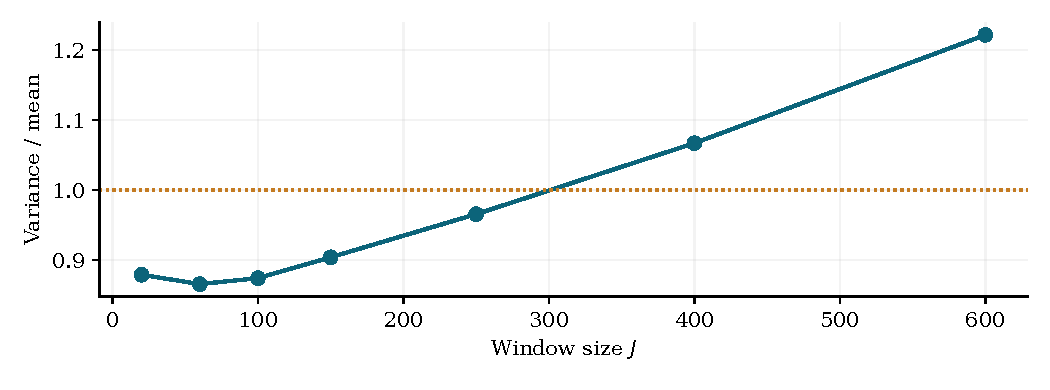
\includegraphics[width=.88\linewidth]{figures/fano.pdf}
\caption{The empirical Fano factor $\operatorname{Var}(V_J)/\E V_J$ crosses 1 between the displayed widths $250$ and $400$.}
\label{fig:fano}
\end{figure}

A plausible source of wide-window overdispersion is the variation of $H(N)$ in \eqref{eq:H} across targets.  The law of total variance gives the exact decomposition
\begin{equation}\label{eq:totvar}
 \operatorname{Var}(V_J)=\E[\operatorname{Var}(V_J\mid H)]
 +\operatorname{Var}(\E[V_J\mid H]).
\end{equation}
If the conditional mean is approximately proportional to $H$, then variation of the singular series inflates the second term. In the prior finite computation, $\mathrm{sd}(H)/\E H\approx0.0832$; with $\E V_{600}\approx27.786$, the naive heterogeneity contribution is $(27.786\times0.0832)^2\approx5.34$, compared with an observed variance-minus-mean of $6.15$. This is a useful numerical explanation, but the proportionality assumption and remainder have not been proved.  Correlation theory for primes in short intervals provides useful conceptual precedents \cite{MontgomerySoundararajan2004}.

\section{A conditional Poisson law}
The first-arrival scaling suggested by the classical Goldbach singular series \cite{HardyLittlewood1923} is
\begin{equation}\label{eq:Z}
 Z(N)=\frac{2C_2H(N)d(N)}{\log^2(N/2)}.
\end{equation}
The approximation $Z\sim\operatorname{Exp}(1)$ was motivated empirically by the earlier first-arrival study, but it is not presently an unconditional consequence of the Hardy--Littlewood conjecture without appropriate uniformity and averaging.

For an asymptotic formulation, choose $N$ uniformly from
\[
 \mathcal N_X=\{N\in[X,2X]:N\equiv10\pmod{60}\},
\]
and, for $x>0$, set
\begin{equation}\label{eq:windowx}
 J_N(x)=\left\lfloor\frac{x\log^2(N/2)}{12C_2H(N)}\right\rfloor,
 \qquad V_x(N)=\sum_{1\le j\le J_N(x)}A_j(N).
\end{equation}
The factor $12$ converts the continuous half-gap $d$ to the lattice index $j=d/6$.

\begin{theorem}[Factorial-moment criterion]\label{thm:poisson}
Fix $x>0$.  Suppose that, as $X\to\infty$, for every fixed positive integer $r$,
\begin{equation}\label{eq:momentassumption}
 \frac1{|\mathcal N_X|}\sum_{N\in\mathcal N_X}(V_x(N))_r\longrightarrow x^r.
\end{equation}
Then $V_x(N)$ converges in distribution to a Poisson random variable of mean $x$, and
\begin{equation}\label{eq:conditionalexp}
 \frac1{|\mathcal N_X|}\#\{N\in\mathcal N_X:Z(N)>x\}\longrightarrow e^{-x},
\end{equation}
provided the exceptional representation $3+(N-3)$ is treated as in the definition of $d(N)$.
\end{theorem}
\begin{proof}
Convergence of all factorial moments to $x^r$ implies convergence in distribution to $\operatorname{Poisson}(x)$ by the method of moments (the Poisson law is moment-determinate).  The event $V_x(N)=0$ is exactly the absence of a nonexceptional representation with positive half-gap $\le 6J_N(x)$, equivalently $Z(N)>x$ when the exceptional endpoint $3$ does not give a closer representation. For sufficiently large $N$, its half-gap $N/2-3$ is much greater than $O(\log^2N)$, so the exceptional representation cannot change this equivalence at any fixed $x$.  The Poisson limit gives $\Prob(V_x=0)\to e^{-x}$.
\end{proof}

\begin{remark}[The unproved arithmetic input]
Hypothesis \eqref{eq:momentassumption} requires uniform control of configurations of $2r$ prime linear forms for every fixed $r$, averaged over many reflected configurations, together with their singular series.  The CRT identities and pairwise correlations alone cannot imply it.  Gallagher's conditional Poisson result for primes in logarithmically short intervals is an influential analogy \cite{Gallagher1976}, but does not supply these reflected-pair moment estimates. Related singular-series averaging problems have been studied in \cite{FriedlanderGoldston1995,GoldstonHuntsNgotiaoco2017}.
\end{remark}

\section{Discussion: what the dynamics does and does not imply}
The observed distribution is compatible with a first-arrival scale $d(N)\asymp\log^2 N$ \emph{in a statistical sense}. At the same time, $\delta_{\min}(N)=2d(N)/N$ becomes small as $N$ grows. Thus the nearest occupied site can retreat from the arithmetic midpoint in absolute units while approaching zero in normalized imbalance space.

The present work separates three distinct levels of information:
\begin{itemize}
\item \textbf{Unconditional arithmetic:} the local forbidden residue sets, the exact finite CRT density \eqref{eq:CRT}, the two-site multipliers \eqref{eq:ratio}--\eqref{eq:attraction}, and the modulo-$7$ exclusion \eqref{eq:forbiddenfour}.
\item \textbf{Reproducible finite evidence:} correlations for $1\le h\le26$, void probabilities, low-order factorial cumulants, and the underdispersion-to-overdispersion transition for targets through $30$ million.
\item \textbf{Conditional asymptotics:} a Poisson law and hence exponential first arrival follow under the explicit all-order factorial-moment hypothesis \eqref{eq:momentassumption}, which is not currently established.
\end{itemize}
No conclusion here rules out isolated even integers lacking Goldbach representations.  Positive local densities, an accurate average model, or a Poisson limit along a density-one set would not themselves exclude a sparse exceptional set.  The next rigorous goal is to bound \emph{uniformly} the averaged errors in the reflected $2r$-prime singular-series sums, or to identify a structural constraint stronger than finite local admissibility.

\section*{Reproducibility and computational protocol}
The supplementary package contains four C++/Python sieve and cumulant programs, the original first-arrival enumeration program, tabulated outputs, and the plot generator (file details appear in the README). C++17 with \texttt{-O3} and Python with SymPy, NumPy, and Matplotlib are sufficient.  The prime sieve extends to $30{,}000{,}000$, the target sample is exactly \eqref{eq:sample}, and the individual correlation plots use indices through $120$.  For the wider-window statistics, indices through $600$ are used.  Reported percentages are empirical frequencies on the specified finite sample.  The author welcomes independent replication and mathematical correction.

\clearpage
\printbibliography
\end{document}
